% The Preamble {{{
%%%%%%%%%%%%%%%%%%%%%%%%%%%%%%%%%%%%%%%%%%%%%%%%%%%%%%%%%%%%%%%%%%%%%
%% This is a (brief) model paper using the achemso class
%% The document class accepts keyval options, which should include
%% the target journal and optionally the manuscript type. 
%%%%%%%%%%%%%%%%%%%%%%%%%%%%%%%%%%%%%%%%%%%%%%%%%%%%%%%%%%%%%%%%%%%%%
\documentclass[journal=jacsat,manuscript=article]{achemso}

%%%%%%%%%%%%%%%%%%%%%%%%%%%%%%%%%%%%%%%%%%%%%%%%%%%%%%%%%%%%%%%%%%%%%
%% Place any additional packages needed here.  Only include packages
%% which are essential, to avoid problems later. Do NOT use any
%% packages which require e-TeX (for example etoolbox): the e-TeX
%% extensions are not currently available on the ACS conversion
%% servers.
%%%%%%%%%%%%%%%%%%%%%%%%%%%%%%%%%%%%%%%%%%%%%%%%%%%%%%%%%%%%%%%%%%%%%
\usepackage[version=3]{mhchem} % Formula subscripts using \ce{}
\usepackage{amsmath}
\usepackage{xcolor}
\usepackage{longtable}
\usepackage{listings}
\usepackage[colorinlistoftodos]{todonotes}
%\usepackage[a4paper]{geometry}
\usepackage{minted}      % code syntax highlighting
\usepackage{soul}        % strike through by \st{text here....}
\usepackage[hybrid]{markdown}

%New colors defined below
\definecolor{codegreen}{rgb}{0,0.6,0}
\definecolor{codegray}{rgb}{0.5,0.5,0.5}
\definecolor{codepurple}{rgb}{0.58,0,0.82}
\definecolor{back}{rgb}{0.95,0.95,0.92}
\definecolor{red}{rgb}{255,0,0}
\definecolor{teal}{rgb}{0,255,255}

%\renewcommand{\lstlistingname}{Chart}
%Code listing style named "mystyle"
%\lstdefinestyle{mystyle}{
%  xleftmargin=4em,
%  xrightmargin=4em,
%  backgroundcolor=\color{white},
%  commentstyle=\color{teal},
%  keywordstyle=\color{red},
%  numberstyle=\tiny\color{blank},
%  stringstyle=\color{red},
%  basicstyle=\footnotesize,
%  breakatwhitespace=false,         
%  breaklines=true, 
%  captionpos=t,                    
%  keepspaces=true,                 
%  numbers=left,
%  numbersep=5pt,                  
%  showspaces=false,                
%  showstringspaces=false,
%  showtabs=false,                  
%  tabsize=2
%}

%"mystyle" code listing set
%\lstset{style=mystyle}
%%%%%%%%%%%%%%%%%%%%%%%%%%%%%%%%%%%%%%%%%%%%%%%%%%%%%%%%%%%%%%%%%%%%%
%% If issues arise when submitting your manuscript, you may want to
%% un-comment the next line.  This provides information on the
%% version of every file you have used.
%%%%%%%%%%%%%%%%%%%%%%%%%%%%%%%%%%%%%%%%%%%%%%%%%%%%%%%%%%%%%%%%%%%%%
%%\listfiles

%%%%%%%%%%%%%%%%%%%%%%%%%%%%%%%%%%%%%%%%%%%%%%%%%%%%%%%%%%%%%%%%%%%%%
%% Place any additional macros here.  Please use \newcommand* where
%% possible, and avoid layout-changing macros (which are not used
%% when typesetting).
%%%%%%%%%%%%%%%%%%%%%%%%%%%%%%%%%%%%%%%%%%%%%%%%%%%%%%%%%%%%%%%%%%%%%
\newcommand*\mycommand[1]{\texttt{\emph{#1}}}

%%% Need this for "Figure S1" labeling, etc.
\newcommand{\beginsupplement}{%
        \setcounter{table}{0}
        \renewcommand{\thetable}{S\arabic{table}}%
        \setcounter{figure}{0}
        \renewcommand{\thefigure}{S\arabic{figure}}%
     }

%%%%%%%%%%%%%%%%%%%%%%%%%%%%%%%%%%%%%%%%%%%%%%%%%%%%%%%%%%%%%%%%%%%%%
%% Meta-data block
%% ---------------
%% Each author should be given as a separate \author command.
%%
%% Corresponding authors should have an e-mail given after the author
%% name as an \email command. Phone and fax numbers can be given
%% using \phone and \fax, respectively; this information is optional.
%%
%% The affiliation of authors is given after the authors; each
%% \affiliation command applies to all preceding authors not already
%% assigned an affiliation.
%%
%% The affiliation takes an option argument for the short name.  This
%% will typically be something like "University of Somewhere".
%%
%% The \altaffiliation macro should be used for new address, etc.
%% On the other hand, \alsoaffiliation is used on a per author basis
%% when authors are associated with multiple institutions.
%%%%%%%%%%%%%%%%%%%%%%%%%%%%%%%%%%%%%%%%%%%%%%%%%%%%%%%%%%%%%%%%%%%%%
\usepackage[final]{hyperref} % adds hyper links inside the generated pdf file
\hypersetup{
	colorlinks=true,       % false: boxed links; true: colored links
	linkcolor=blue,        % color of internal links
	citecolor=blue,        % color of links to bibliography
	filecolor=magenta,     % color of file links
	urlcolor=blue         
}


%%% HELPER CODE FOR DEALING WITH EXTERNAL REFERENCES
\usepackage{xr-hyper}
\makeatletter
\newcommand*{\addFileDependency}[1]{
  \typeout{(#1)}
  \@addtofilelist{#1}
  \IfFileExists{#1}{}{\typeout{No file #1.}}
}
\makeatother


%%%%%%%% Title %%%%%%%%
\title{A Markov State Model of Solvent Features Reveals Water Dynamics in Protein-Protein Binding}
\author{Robert M. Raddi}
\author{Vincent A. Voelz}
\affiliation[Temple University]
{Department of Chemistry, Temple University, Philadelphia, PA 19122, USA}
\email{voelz@temple.edu}
%\date{Date}

% }}}

\begin{document}
% !TEX root = ./main.tex

\section{Abstract}

In this work, we investigate the role water molecules have in the
binding reaction of p53 transactivation domain to the hydrophobic pocket
of MDM2.~ MDM2 provides negative regulation of the tumor suppressor p53
by binding to the intrinsically disordered N-terminal transactivation
domain (TAD), initiating ubiquitination, and ultimately degradation, of
p53.~ Previously, our group generated 831 µs of explicit-solvent
aggregate molecular simulation trajectory data for the MDM2-p53 peptide
binding reaction using large-scale distributed computing, and
subsequently built a Markov State Model (MSM) of the binding reaction \cite{zhou2017bridging}.
 Upon obtaining solvent features, the MSM construction reveals the
slowest motions in de-wetting, which coincide with the previously
acquired conformational degrees of freedom. The solvent shells
contributing most to the first eigenvector of the time-lagged
correlation matrix (along tIC\textsubscript{1}) are centered on T18 of
p53 and H73 of MDM2, in the ranges of (3-6) Å and (0-3) Å, respectively.
In atomic detail, trajectories of 'important' solvent shells were traced
to present a visual representation of these associated water bundles
departing the pocket at discrete occasions.~ Averaging instantaneous
water density over all snapshots for tIC1 and tIC2 clarifies binding
mechanism as well as reaffirming the hydrophobic effect.


% !TEX root = ./main.tex

\section{Introduction}


Tumor suppressor protein p53 is regulated by the E3 ubiquitin-protein
ligase MDM2, which binds the transactivation domain (TAD) of p53 and
recruits it for degradation. Whereas p53 TAD is intrinsically
disordered, it forms a helix upon binding to MDM2.

There has been great interest in using molecular simulation to probe the
mechanisms for this association. Molecular dynamics (MD) has become a
vital tool and is especially useful for understanding the binding
mechanism of proteins. Many MD simulations have previously been used to
study the protein-protein interaction of the MDM2-p53 system, and the
focal point of these results suggest an 'induced-fit', or `fly-casting'
mechanism, in which binding of p53 to MDM precedes folding to a
well-structured helix.

In all of the previously published work on the MDM2-p53 system, there
has been surprisingly subtle insight on the role water plays. It has
been suggested from Marie-Claire et al \cite{bellissent2016water} and many others \cite{spyrakis2017roles,yang2013approaches} that
solvent and protein motions may be interconnected, and the dynamics of
the protein is ``slaved'' to the solvation layers. It could be argued
that protein function, conformational dynamics and stability are all a
result of solvent dynamics. The main driving force underlying protein
folding and binding is the hydrophobic effect, which is mediated by
water. Indeed, explicit-solvent molecular simulations are typically
dominated by large numbers of water molecules.

Normally, molecular simulation studies investigate protein
conformational features, where hydrophobic interactions dictate the
slowest motions. To what extent would it possible to examine protein
binding dynamics using only solvent degrees of freedom? In this work,
our goal is to determine what role water plays in the protein binding
mechanism, particularly in the binding pocket of MDM2 when p53 binds.

To uncover the specificities of water-protein interactions, here we
explore methods to transform the positions of solvent molecules in
molecular simulations to quantifiable features that can be used to build
Markov State Models (MSMs) of conformational dynamics. A Markov State
Model is a network of conformational states and transition rates
connecting them \cite{schwantes2014perspective,bowman2013introduction}. In practice, an MSM is constructed by
estimating a transition probability matrix from the trajectory data,
which determines the likelihood of transitioning from one state to
another in some small time interval.

A crucial step in constructing an MSM is discovering the relevant
metastable states, which for large trajectory datasets requires
conformational clustering, typically done concurrent with a dimensionality
reduction method such as time-independent component analysis (tICA).
tICA is a statistical model that performs a dimensionality reduction by
eigendecomposition of the time-lagged correlation matrix,
\emph{C}\textsuperscript{∆\emph{t}}, which finds the coordinate vectors
along which conformational motions decorrelate most slowly. \cite{bowman2013introduction}

Below, we describe the process of building an MSM of the p53-MDM2
binding reaction using only solvent coordinates, from a previously
published trajectory dataset \cite{zhou2017bridging} of more than 900 µs of aggregate
simulation time in explicit solvent. Thus, our work offers an
unprecedented opportunity to examine the role of solvent in
protein-protein binding.


% !TEX root = ./main.tex

\section{Methods}

\textbf{Molecular Dynamics}

Molecular simulation trajectories of \emph{ab initio} peptide binding
were performed on Folding@home (FAH) (7) using Gromacs 4.5.4 (8) with
TIP3P explicit solvent and the Amber ff99sb-ildn-nmr force field, as
described by Zhou et al (1). The protein data bank (PDB) denotes the
well-known MDM2-p53 system as 1YCR. Initial atomic coordinates from 1YCR
were used as a template in the production of approximately 976 µs of
aggregate simulation data.

\textbf{Solvent Shell Featurization}

Previously, the analysis of trajectories consisted of strictly protein
conformational degrees of freedom (DOF). Pair distance features between
C\textsubscript{α} and C\textsubscript{β} atoms of selected residues
(see Supplementary Materials) positioned within the binding region of
MDM2 and p53 were used. In contrast to the distance metric between
C\textsubscript{α} and C\textsubscript{β} atoms in Zhou's work, each
trajectory was described by the "SolventShellFeaturizer'' tool for
MSMBuilder (9).

Solvent features are a collection of all the water oxygens that had been
binned in accordance to their respective shell occupancies.
``Important'' water atoms are defined as the solvent atoms located in
the union of two or more shells with differing solute atoms. Parameters
for the solvent shell featurization followed the optimization determined
by Harrigain et al., (9) which encompasses the use of four solvent
shells around each solute atom with a shell width equal to 3.0 Å each.

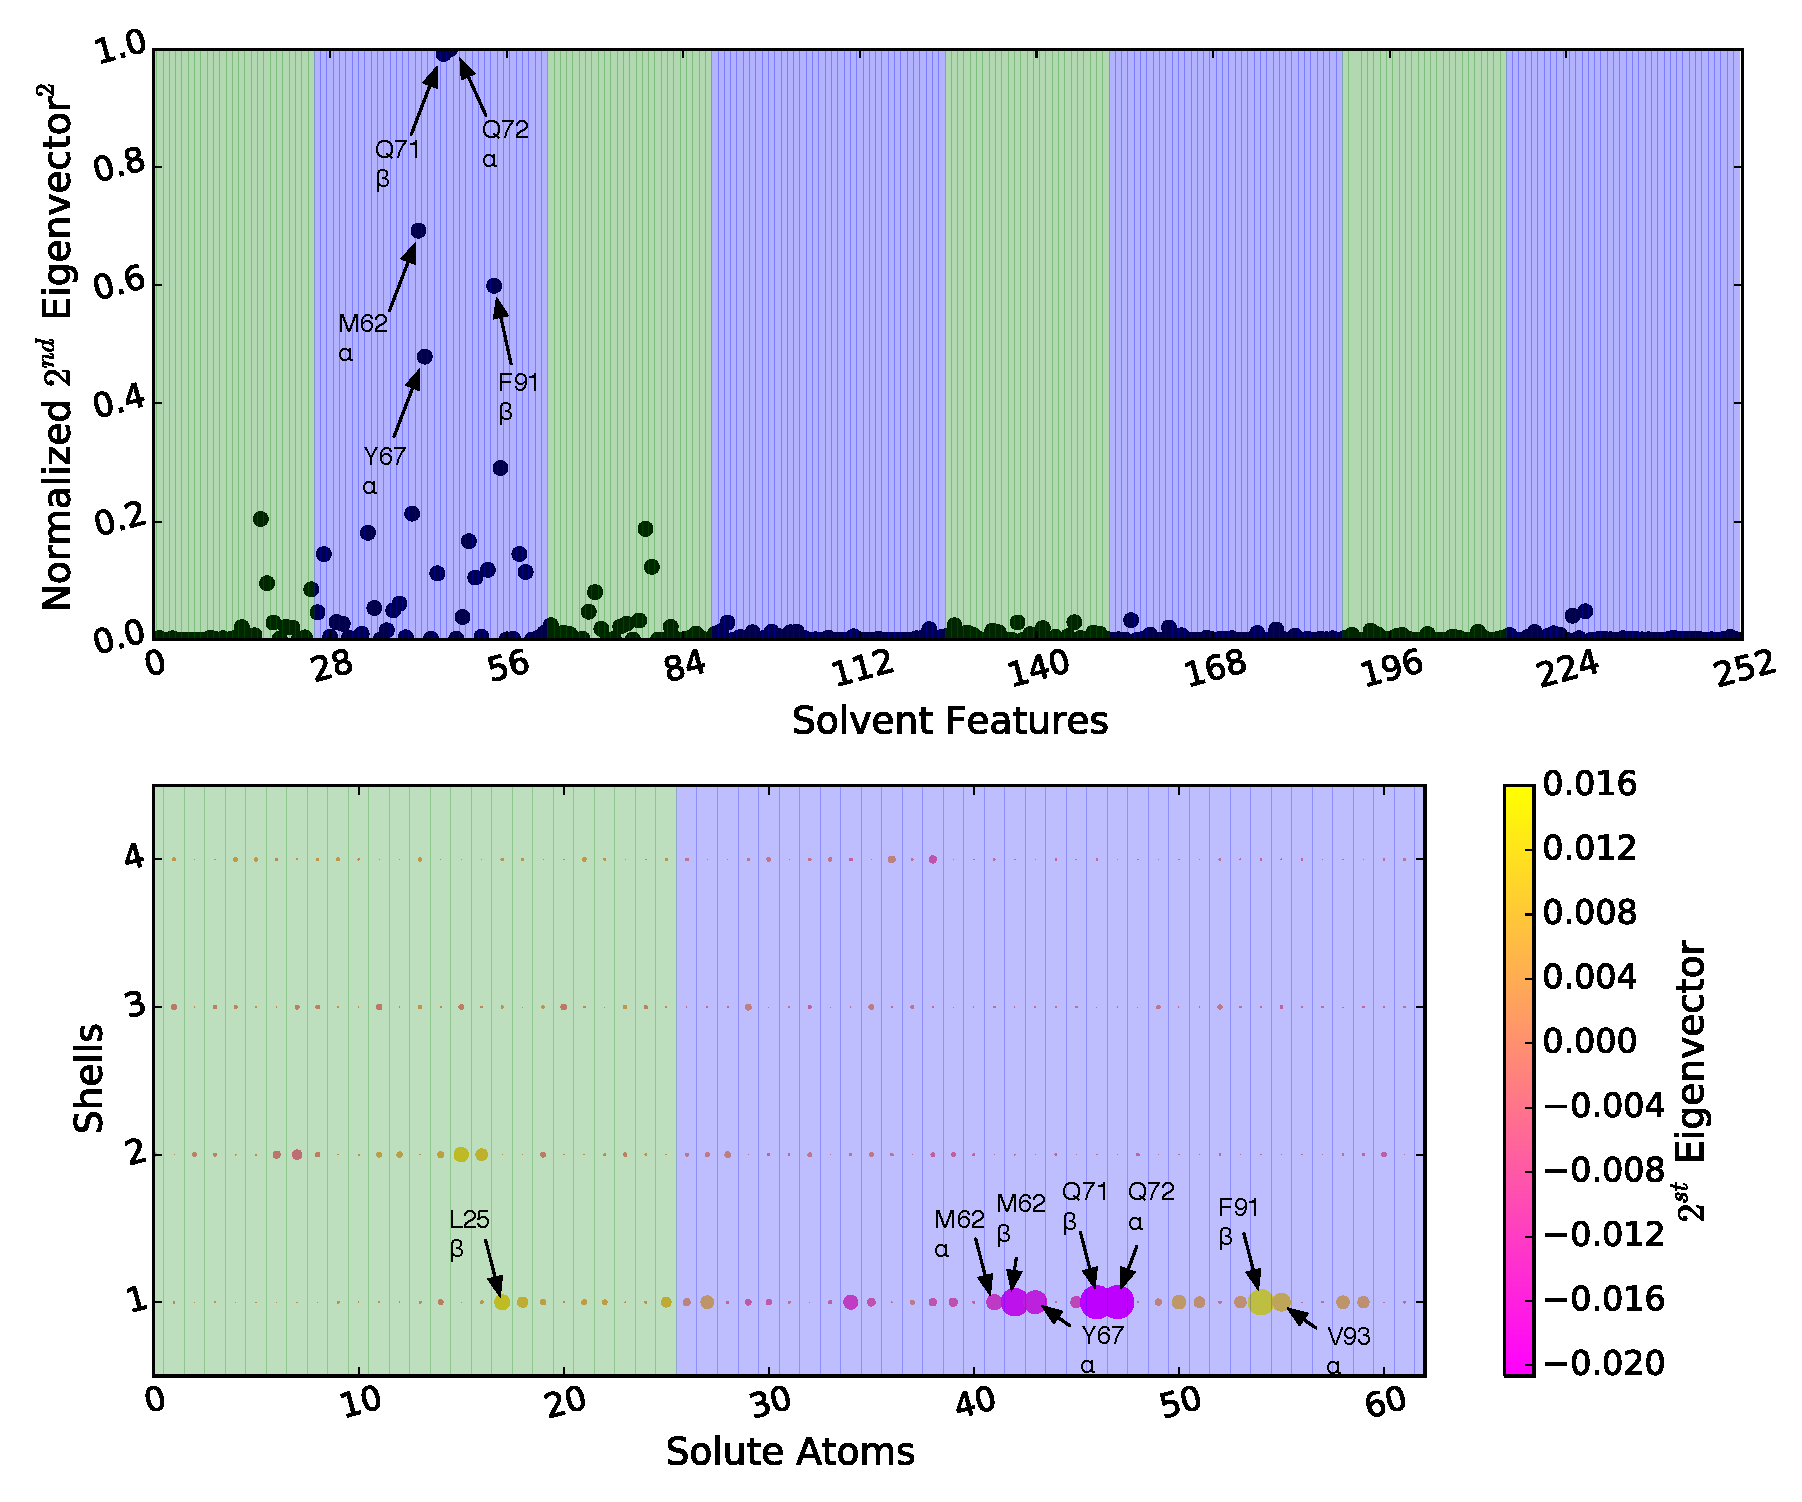
\includegraphics[width=6.5in,height=2.29097in]{media/image1.emf}

\textbf{Figure 1.} "Solvent Shell Featurization" provides location of
specific solvent shell features by binning solvent atoms (blue circles)
according to specific solute atoms (green circles) with respect to shell
index. ``Important'' solvent features are highlighted red, which are
defined by solvent atoms residing within overlapping shells (gray
shading).

\textbf{MSM construction}

In recent years, MSMs have proven to proven to be a strong tool in many
sectors of biophysics, including protein folding (10, 11),
conformational dynamics (1), as well as solvent dynamics (9). We
describe solvent dynamics using WetMSM (9), MDTraj (12) and MSMbuilder
(13) libraries. Using the latter python libraries, linear combinations
of solvent features were used to compute a new basis set, the tICA
subspace. The eigenvectors of the tICA time-correlation matrix relate to
the degrees of freedom associated with the conformational change (6).
Hence, the metastability of specific solvent shells contributing to the
slowest de-wetting processes were determined from the eigenvectors
correlated with the slowest relation timescales.

Previous tests suggest (14) that 10 tICA components with 600 microstates
and a 5 ns lagtime is best suited for the construction of the
protein-only tICA model. In order to compare protein and solvent MSM's,
the tICA parameters remained the same in the wetMSM (9) construction.

\textbf{MolMap }

Chimera's molmap (16) function allows for visualization of specific
water density within trajectories. Appling this volume density map
technique provides an unparalleled visualization of ``important''
solvent-protein interactions. All water-oxygens for each snapshot were
selected when computing the density surface. The initial contour level
to enclose a fraction of the total mass was set to 0.9895 and the grid
spacing to 1.3. The volume contour level was then changed to 0.015 to
apply Gaussian filtering. Gaussian filtering was performed for each
individual surface in order to reduce the amount of flickering when
moving from snapshot to snapshot.



% !TEX root = ./main.tex

\textbf{Results}

\textbf{Complementary Transitions Implies Hydrophobic Effect}

How do MSMs from solvent coordinates match up with the protein centric view? Solvent and protein transitions are found to be interconnected, such that when mapping each set of input features to the first two slowest-relaxing tICA components there exists overwhelming similarities. Potential energy wells overlap for the two largest tICA components, tIC1 and tIC2. Furthermore, the metastable states that correspond to these basins are identical for both tICA landscapes. Many have proposed various roles for water molecules, such as water enslaving protein motions \cite{bellissent2016water}. Here, in fine detail the latter proposal was scrutinized by exposing the solvent shells that contributed to the slowest motions in the de-wetting process and emphasizing theconsequence of solvent density within the binding site.

Previously, the protein centric viewpoint of binding has been revealed. In this work, we reconstructed the protein centric MSM and built an MSM using solvent features to investigate the role of water. The same model parameters were used to objectively compare our models. A side-by-side comparison of the two tICA landscapes can be found in Figure \ref{fig:tica_compare} and implied timescales in Figure \ref{fig:implied_timescales}. The first model was built from protein pair-distances and the other using a solvent shell features metric. Remarkably, by randomly extracting clusters from the tICA subspace (Figure \ref{fig:tica_compare}) at each quadrant, we revealed that the four main metastable states coincide with findings from Zhou et al. and are as follows: top left represents the unbound-unfolded, bound-unfolded in the top right, bound-folded in the bottom right, bottom left is the bound-unfolded.

The similarities do not end here. The correlation with Tryptophan, W23 of p53, and tIC2
still exists in the solvent MSM. It has been found that trajectories that start at (+tIC1, +tIC2), and finish at the native state (+tIC1, -tIC2) predominantly display W23 facing out of the page when looking at MDM2-p53 from the orientation shown in all the figures from this work. Likewise, trajectories starting at (-tIC1, -tIC2) show W23 oriented into the page.  An observed trend impossible to detect from the protein centric model shows that post binding of MDM2-p53, bundles of water is commonly found to associate—requiring an increase of water fluctuation to induce burrowing of W23.


The second component (tIC2) is related to the first component, which directly corresponds to de-wetting. When moving from -tIC1 to +tIC1, we find a
direct correlation in the number of water molecules inside the pocket, corresponding to the proximity of p53 to MDM2's binding site, where the location of the native state resides in (+tIC1,-tIC2) of the tICA landscape. Naturally, as bulky residues enter the hydrophobic pocket, water tends to relocate to find more polar interactions. For example, as greasy tryptophan (W23) enters the pocket with or without the correct orientation, there is a positive shift along tIC1, and stability of the bound alpha helix is maximized when W23 is in the correct orientation (into page). Phenylanine (F19) also induces a positive shift along tIC1 as it buries regardless of W23's orientation (+tIC1, ±tIC2).

\textbf{Slowest-dyanmical Solvent Features}

Solvent shell featurization achieves instantaneous solvent density with
respect to solvent features over all trajectories \cite{harrigan2015conserve}. Solvent features are binned water molecules from considering only solute-solvent distances. The 63 solute atoms ($C_{\alpha}$'s and $C_{\beta}$'s) each contain 4 equidistant shells around them giving 252 solvent features.
%Information regarding specific shells must be taken from the eigenvector, which requires decomposition to investigate each of the shells with respect to specific solute atoms.
The feature vector yields information over all trajectories and was transformed by tICA to produce a linear combination of water features. After construction of the 10-component tICA model, which serves as the new basis set for the data, we subsequently built a
solvent MSM following equivalent parameters as Zhou et al.

Information regarding individual solvent features that correlate to the slowest-dynamical motions of de-wetting were extracted from the 1\textsuperscript{st} eigenvector. From this, mechanism is determined.  The important solvent features are represented as a color map shown in the bottom panel of Figure \ref{fig:1st_eigenvector}, moving from negative (pink) to positive (yellow).  The color represents the degree of contribution to the slowest dynamical solvent motions within a specific shell. The coefficients used to represent this magnitude comes from the normalized 1\textsuperscript{st} eigenvector to elude from noise (top panal of Figure \ref{fig:1st_eigenvector}).


The residues with the greatest contributions to the slow motions of de-wetting are shown in Figure \ref{fig:atom_indices} and have been colored accordingly for a convenient reference.  The slow-dynamical solvent features included the first shell (0-3 Å) of Histidine, H73 ($\alpha$) and Glutamine, Q72 ($\alpha$, $\beta$) of MDM2 along with the second shell (3-6 Å) of K24($\alpha$, $\beta$) and T18($\alpha$, $\beta$) of p53.




\begin{figure}[h!]
\centering
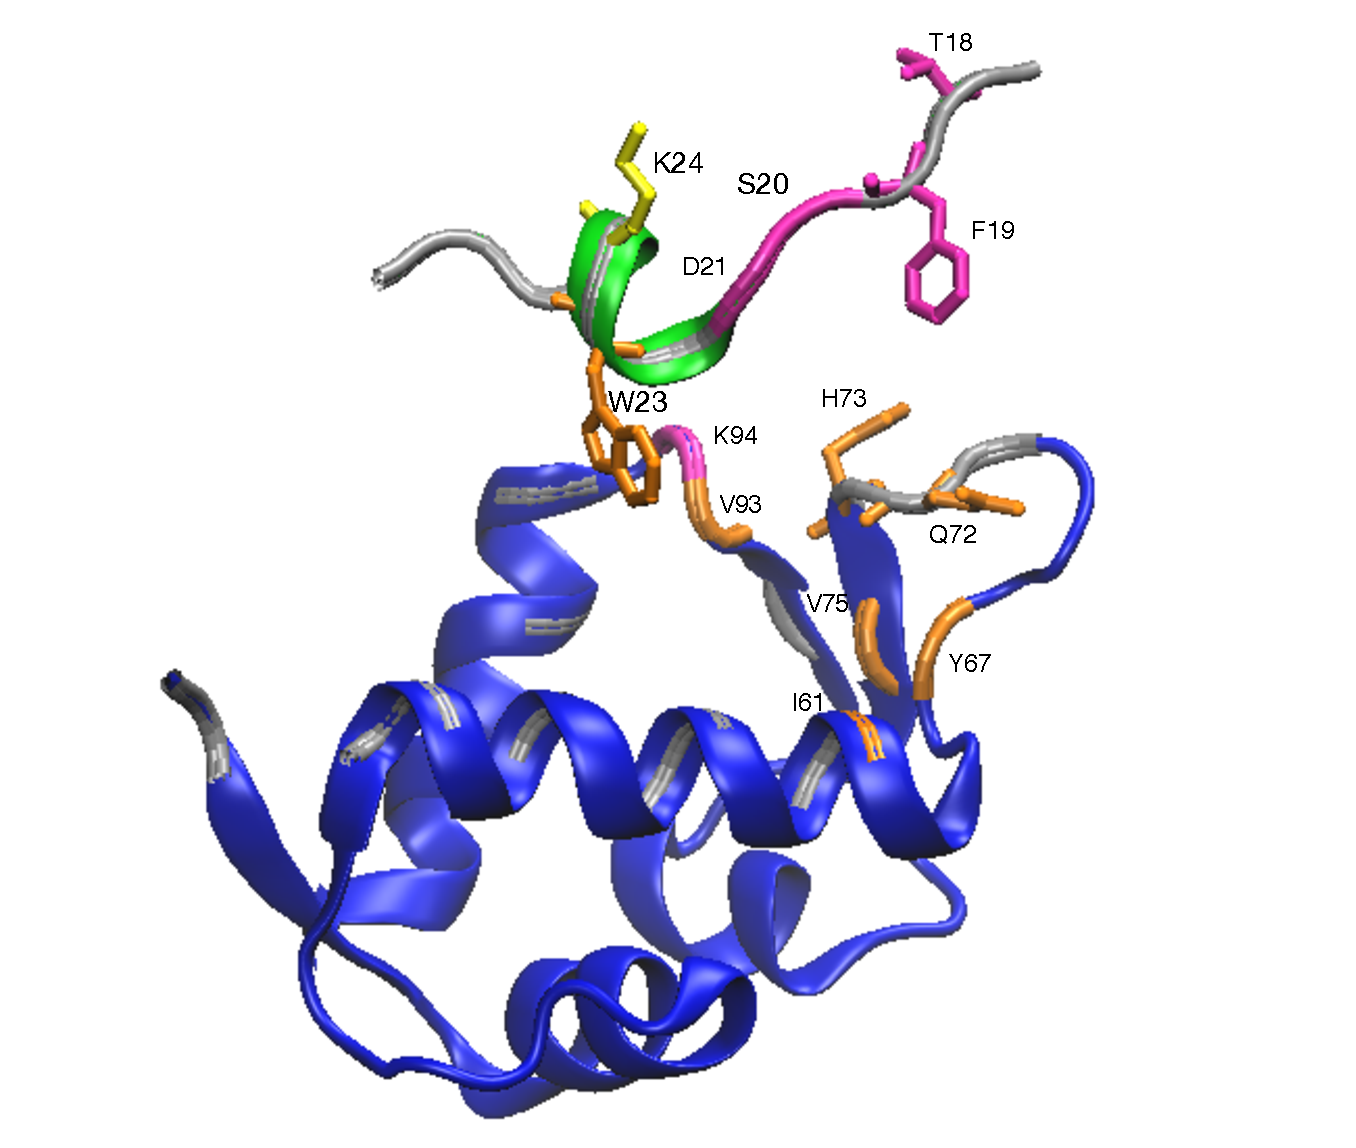
\includegraphics[scale=0.5]{Figures/Structure/Atom_indices_with_1st_eigenvector_sel.pdf}
\caption{MDM2 (blue) and p53 (green) shown with residues (silver, orange, pink, and yellow) containing $C_{\alpha}$ and $C_{\beta}$ solute atoms selected for water shell featurization. Significant residues are identified from the normalized squared components of the 1\textsuperscript{st} eigenvector (see Figure \ref{fig:1st_eigenvector}) and colored accordingly.}
\label{fig:atom_indices}
\end{figure}


\begin{figure}[h!]
\centering
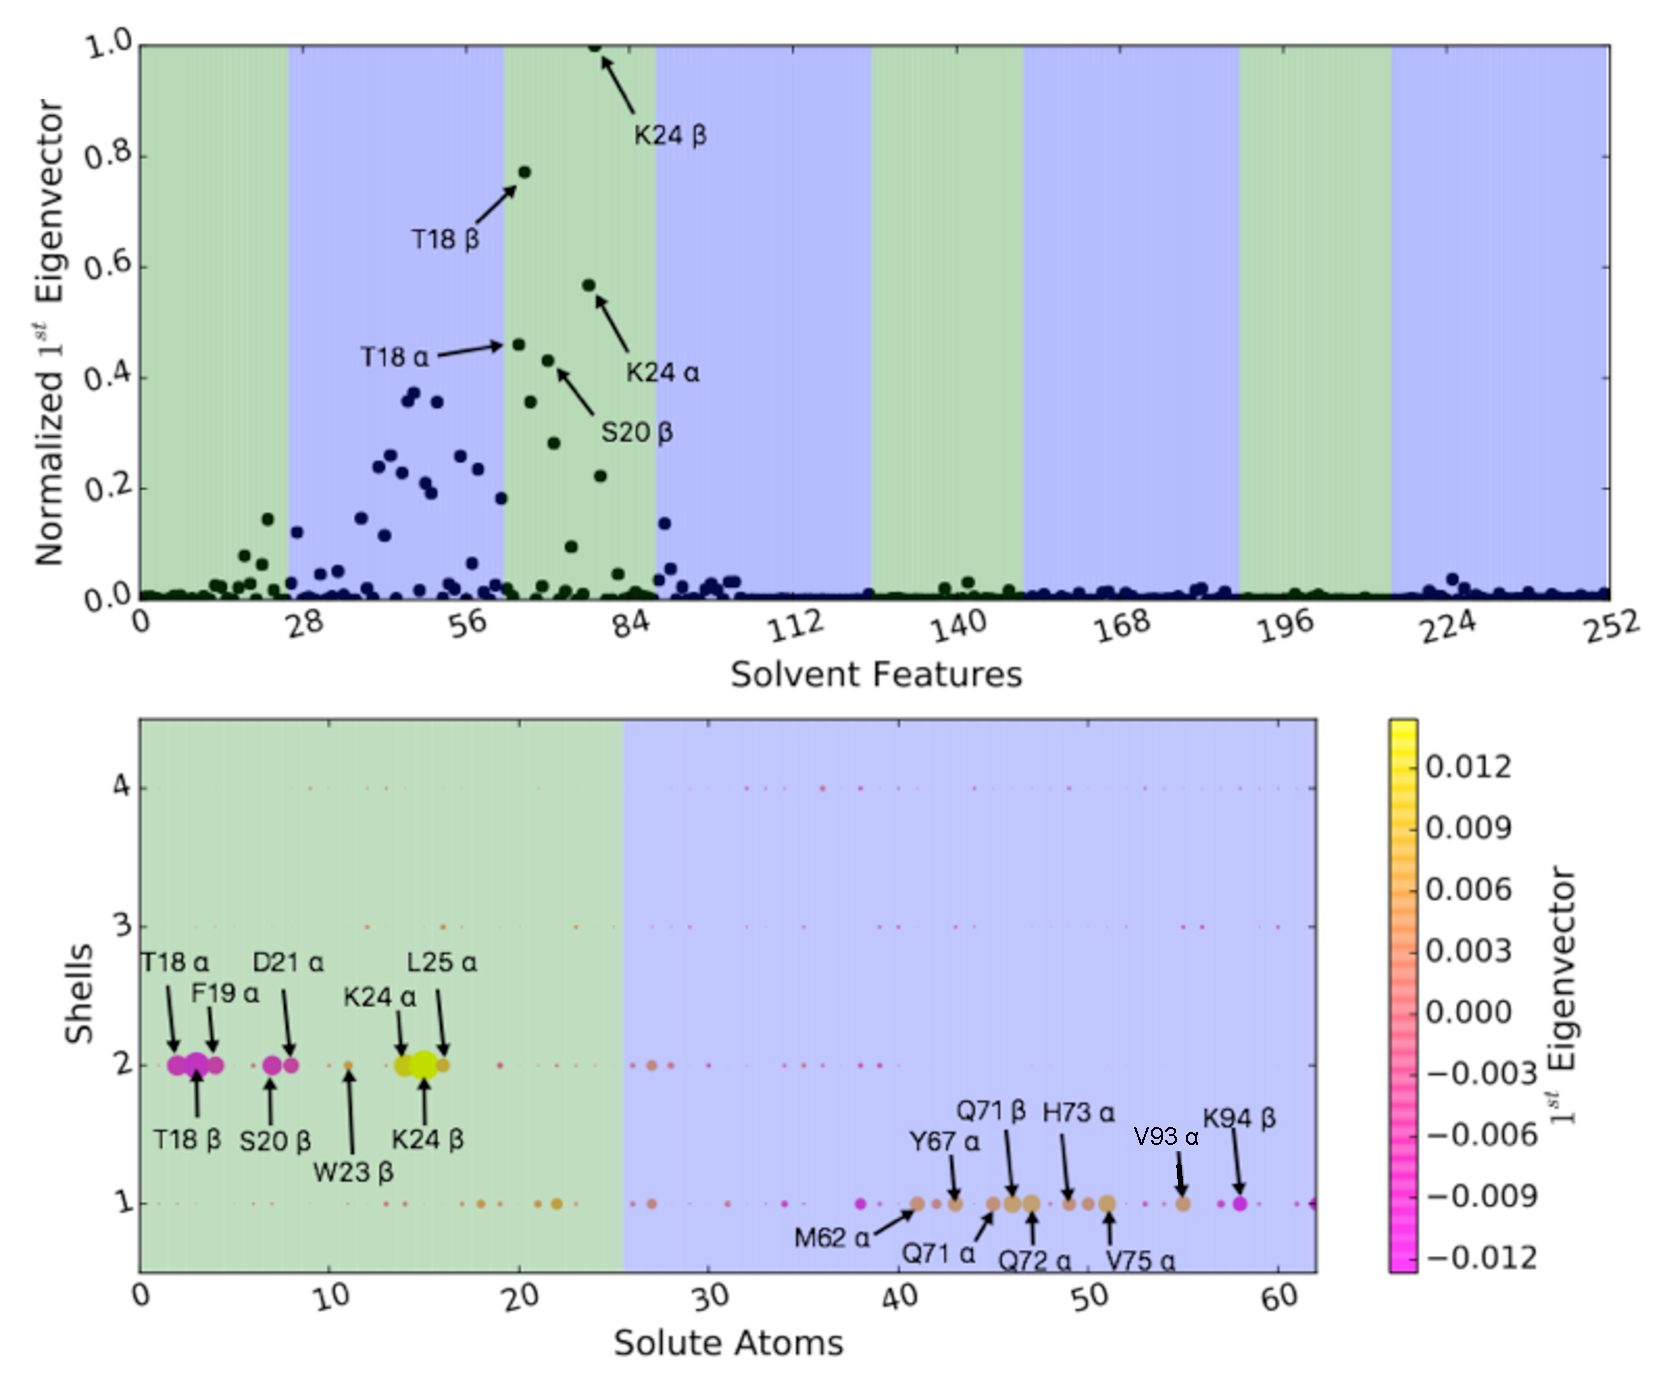
\includegraphics[scale=0.5]{Figures/SolvShellFeatures/Solvent_Shell_Feature_Eigen_1.pdf}
\caption{\textbf{Solvent shells around key residues contribute to the slowest de-wetting motions.} (Top) The degree of contribution for each solvent shell. Significant slow-dynamical solvent features are labeled for important solute atoms ($C_{\alpha}$ and $C_{\beta}$). The first 26 features are of the first shell of p53 (green), then the next 38 are of the first shell of MDM2 (blue). Next, second shell of p53, and so on. (Bottom) Transformed eigenvector to show individual shell contribution. The color map represents the slow solvent dynamics of the system as it relaxes towards equilibrium (pink to yellow).}
\label{fig:1st_eigenvector}
\end{figure}


Using the solvent shell metric associated with the greatest magnitude of importance (3-6 Å of p53) the waters within this region were highlighted and traced along specific trajectories. In addition to this quantitative approach, instantaneous (1 ns) solvent density was qualitatively uncovered with the help of Chimera's MolMap. At each instant along a trajectory an occupancy surface was gen rated to clearly represent the absence of water-oxygens. As one would expect, an inverse relationship was found for the proximity of p53 to MDM2 and the number of water-oxygens in the vicinity of the pocket.

The tICA landscape in Figure \ref{fig:tica} was generated with solvent shell input features. Overlaid on this 2-D landscape is a trajectory with a duration of 531 ns that spans the majority of tIC1. This particular trajectory undergoes five transitions (a)-(e) where each transition is represented with a snapshot that has been hand selected from the 600 clusters. See the supplemental information section for this trajectory, as well as five additional trajectories (movies) which span all of the quadrants of the tICA landscape.

Four main transition states can be seen in this trajectory, starting from the bound-unfolded ending up into the bound-folded state. This trajectory is consistent with the "fly-casting" mechanism, in that threonine, T18 (cyan) and phenylanine, F19 (light green) of p53 enter the pocket first displacing some transient water molecules, but large surface cavities still exist (a-b). The next transition state (c) occurs at 201 ns (00:07) where W23 (yellow) enters the pocket. Here, expropriation of space by bulky Tryptophan of p53 displaces a large water cluster from the pocket forcing reorganization of water molecules (c). It is the fluctuation of water that assists W23 for a deep insertion into the pocket at 308 ns (00:10). In turn, p53 is pulled down which contorts the alpha helix with a torque screw motion throwing threonine T18 upwards, (d) simultaneously enabling F19 to dig down into the cleft at 314 ns (00:11). In the last transition (e), F19 and W23 hold a strong foundation and maintain alpha helix stability by hydrogen bonds. Solvent eventually makes the environment around K24 chaotic enough to complete the loop for a complete fully structured alpha helix.

\begin{figure}[h!]
\centering
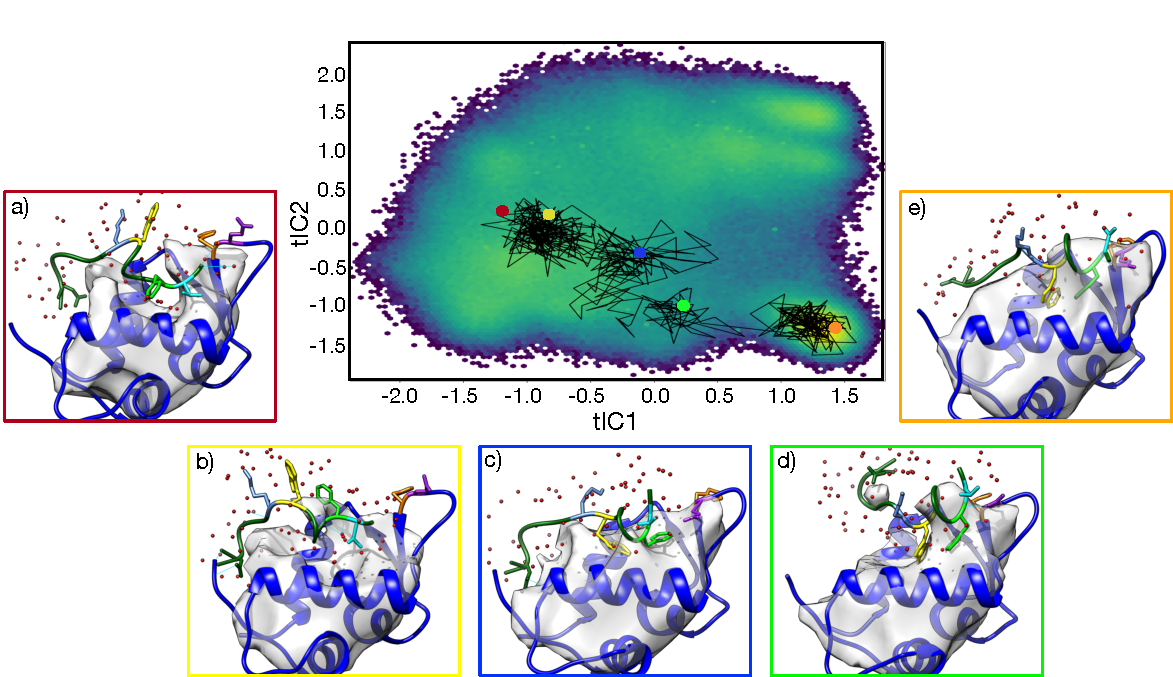
\includegraphics[scale=0.75]{Figures/Partitioned/Partitioned_final.pdf}
\caption{\textbf{De-wetting in a protein binding trajectory.} Solvent
features projected onto a 2D tICA subspace corresponding to the first
and second components, tIC\textsubscript{1} and tIC\textsubscript{2}.~
Each color-coded snapshot represents a transition state containing its
own unique molmap (Gaussian smoothing at the 0.015 level) characterizing
instantaneous solvent density. MDM2 (blue): Q71 (purple), H72 (orange)
and p53 (green): L24 (light blue), T18 (red), F19 (pink) and W23 (cyan).}
\label{fig:tica}
\end{figure}


Water traces are displayed below for T18 and W23 of p53, which have been deemed important residues, more specifically, the 2\textsuperscript{nd} shells of each are regarded significant.  Water traces fro W23 and T18 are shown for the trajectory overlaid in Figure \ref{fig:tica}.  These water counts demonstrate that the transition from (b) to (c) are indeed coupled.


\begin{figure}[h!]
\centering
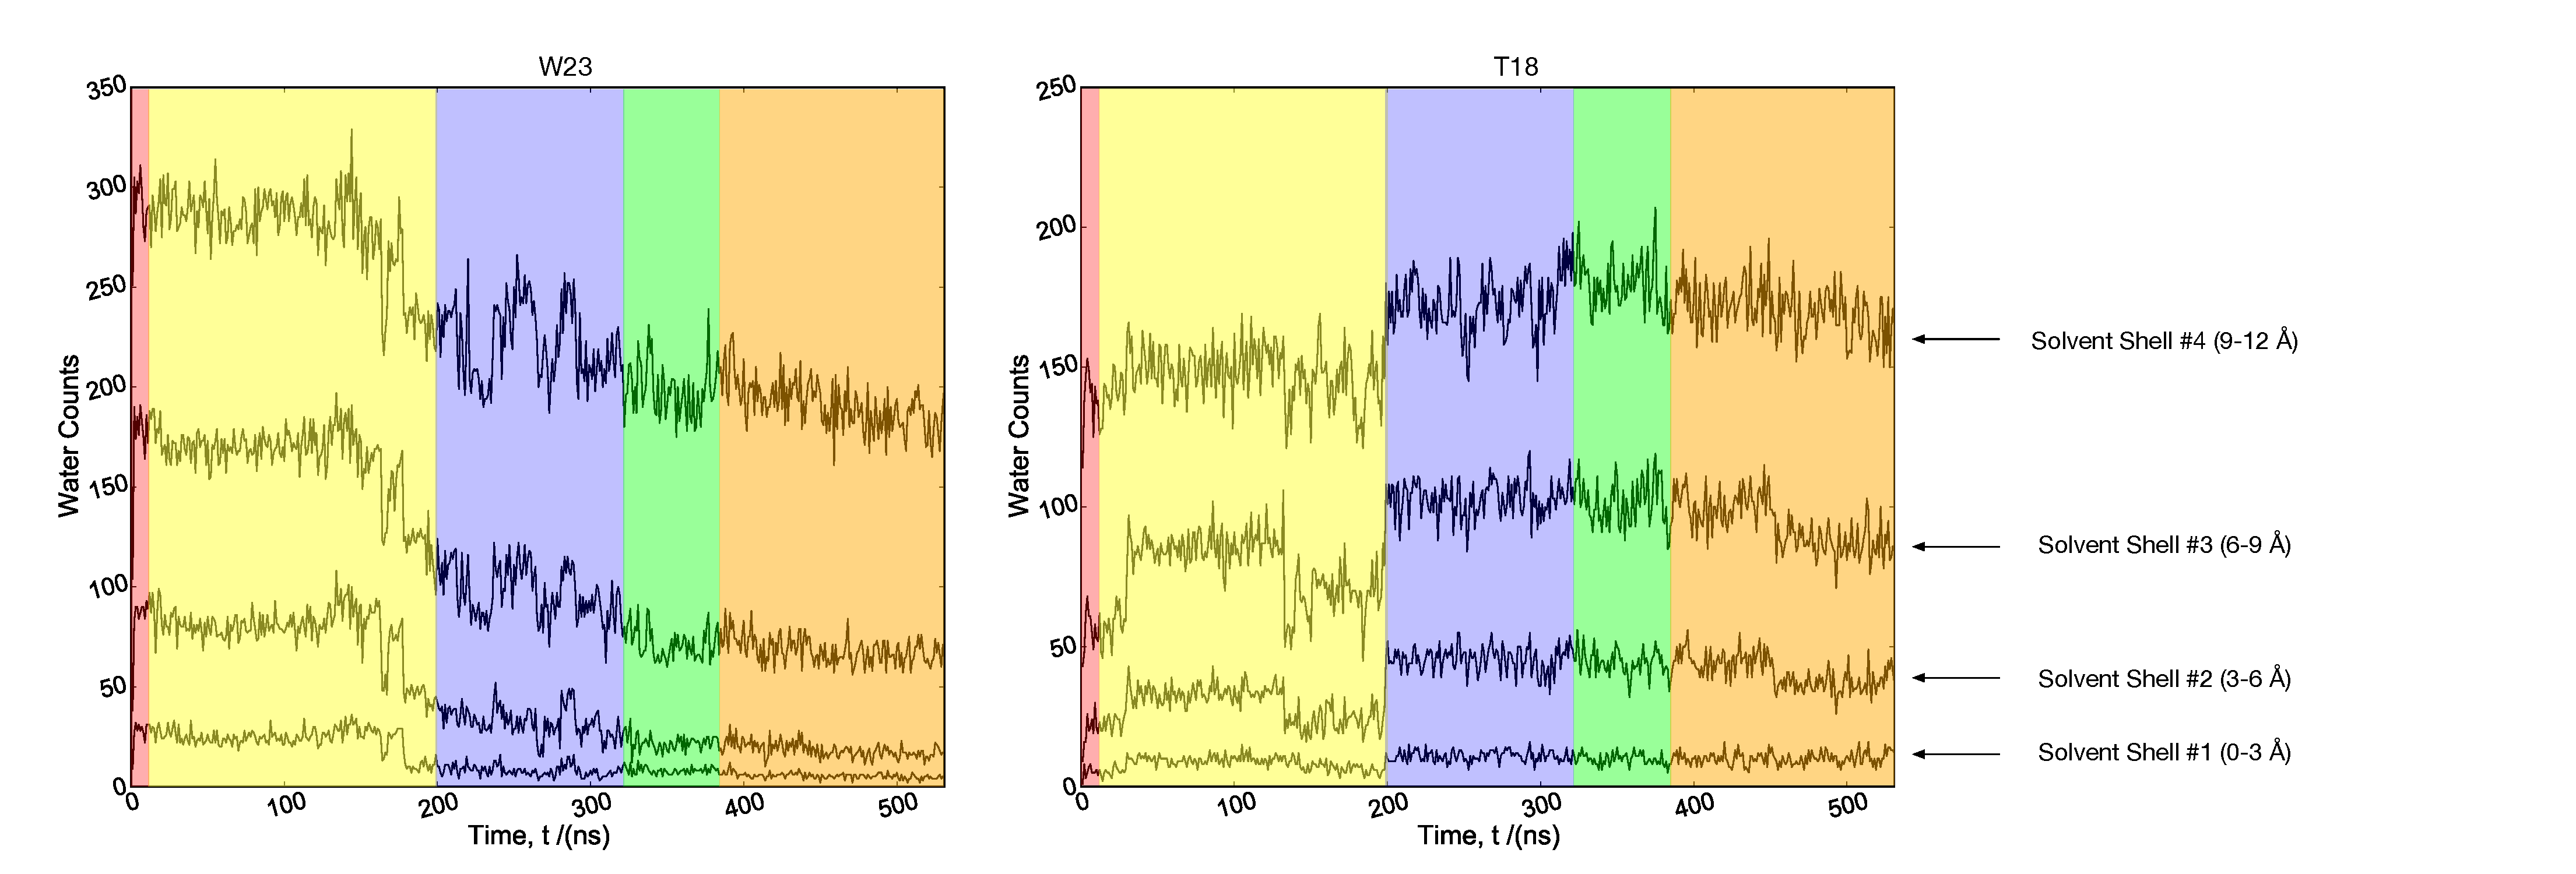
\includegraphics[scale=0.25]{Figures/Water_counts/Water_counts.pdf}
\caption{Water counts for W23 and T18 of p53 TAD,
corresponding to the trajectories shown in Figure 4. Changes in. these
observables discernibly follow the movements associated with transitions
(b)-(d).}
\label{fig:water_counts}
\end{figure}

%T18 was identified to contain significant solvent dynamics around 3-6Å.

%Instantaneous solvent density from specific movies (SI) suggests the hydrophobic effect plays a keyrole in water dynamics.

Interestingly, a recent study \cite{yadahalli2019kinetic} also notes the importance of theronine in the binding of p53 to MDM2 and suggests a ten-to twenty-fold decrease in binding affinity when Thr18 is phosporylated in comparison to the wild-type p53.  It is known that the hydrogen bond acceptor from the oxygen atom in water molecules is in fact a primary mechanism of protein stability. As an example of this, threonine T18 of p53 creates hydrogen bonds with water especially when T18 is in close proximity to Q72 of MDM2, where the jostling of water clusters back-and-forth between these two residues increases the formation of hydrogen bonds.  Water could act as an intermediate state stabilizer if found where hydrogen bonds are formed with the hydroxyl group of polar residues like T18 and Lysine, K24 to facilitate the structural transformation of the p53 $\alpha$-helix. Water bundles are found during important motions of helix formation and can be found looking for surface cavities. Scattering of water leads to reorganization to increase polar interactions and position themselves to a more favorable location.











%It is well known that water can become trapped in cavities as a result of protein binding attempts. Many transitions were found that during the binding of p53-MDM2 water would become trapped inside the hydrophobic pocket. Entrapped waters don't usually vacate until bulky nonpolar residues such as W23 and F19 of p53 form a greasy surrounding for the water molecules slip out.





% !TEX root = ./main.tex

\section{Discussion}

%Take action to prevent criticism {]}}

%\textbf{{[} Talk about any filled gaps, and how this is relevant to the field. {]} }


The WetMSM Solvent Shells Featurization enables instantaneous solvent density over all the trajectories.  This featurizer permits the analysis of MD trajectories from an entirely different viewpoint. We were able to uncover the slowest motions of the system involved in de-wetting and show the effects of water in protein dynamics reaffirming the hydrophobic effect.  Many follow the notion that hydrophobic interactions have the greatest influence of conformational change protein binding, and it is common practice to remove water after simulations to reduce the computational cost of analysis.

Solvent Shells Featurization has the potential to be extremely useful for analyzing water and ions inside a membrane system, sugars involved in hydrogen bonding, or looking at the effects of trapped water bundles in various cavities, which is pertinent to drug design.  It is possible to  uncover substantial detail when turning to this solvent centric point of view.

Deciding what the best features are can be a daunting task, but an important one. A recently developed method by George A. et al. \cite{george2020laplacian} automates the feature selection problem by using the generalized matrix Rayleigh quotient (GMRQ) to objectively decide the optimal featurization for the system. This promising approach will be explored in future works.


\textbf{Did you use any other metric besides strictly protein-protein degrees of freedom or strictly a solvent shell features?} \textbf{Is there a need to use a protein-solvent feature union metric?} Information of both metrics are very similar. It would be unnecessary to perform a computation with a union of protein-solvent features as the comparison of solvent only and protein only features reveal almost identical tICA landscapes. Building Markov state models for both the protein and solvent MSMs with the same parameters show that the differences between the two are strictly in the slowest motions, where the landscape from the solvent model that tIC1 correlates to the slowest de-wetting motions. Contrary to the solvent model, the protein model uncovers the slowest protein motions where Trp of p53 is very important.

\textbf{If tryptophan of p53 is so important to these trajectories, why don't we see it in the solvent shell analysis as being more prominent?}  From the protein-centric model, W23 is found to have great importance.  It is interesting to see that tryptophan is not given the regarded with the same level of importance  when using solvent features. We know that the features deemed significant by tICA are those that have the rare solvent transitions.  In the analysis shown above, W23 was indeed important and can be seen in Figure \ref{fig:water_counts} as it facilitates water fluctuations that effect other residues such as threonine and phenylanine of p53 which have been found to play a very important role in the anchoring and stability during the binding process \cite{zwier2016efficient}.




% collective variables that combine solvent shell features that indicate the rare transitions
%slow directions and rare transitions in the set of basis functions











% !TEX root = ./main.tex

\section{Conclusion}

Using \textasciitilde{}976 µs of trajectory data simulated in explicit
solvent, an MSM of p53-MDM2 binding was constructed via solvent shell
features, offering a complementary, solvent-based view of protein
conformational dynamics. We find that the solvent feature-based MSM
exhibits a landscape very similar to that found in a previously
published MSM constructed from MDM2-p53 protein atom pair distances.
Calculating instantaneous water density over all trajectories ultimately
revealed that the largest contributions to solvation and de-wetting
during the binding are within \textasciitilde{} (3-6) Å of Thr18 and
Lys24 of p53.~The significance of Thr18 in the binding dynamics arises
from its reorganization in the binding site to maximize polar
interactions with water.~ Lastly, the hydrophobic effect was reaffirmed
and visually displayed in atomic detail, using water density surfaces to
illuminate water mediation and water clusters leaving the binding site.


\bibliographystyle{plain}
\bibliography{references}
% !TEX root = ./main.tex


\section{Supplemental Information}


\subsubsection{Methods}
Atom indices for the $C_{\alpha}$'s and $C_{\beta}$'s of the following selected residues of p53 and MDM2, respectively: [Glu-17, Thr-18, Phe-19, Ser-20, Asp-21, Leu-22, Trp-23, Lys-24, Leu-25, Leu-26, Pro-27, Glu-28, Asn-29]; [Glu-25, Thr-26, Met-50, Lys-51, Leu-54, Leu-57, Gly-58, Ile-61, Met-62, Tyr-67, Gln-71, Gln-72, His-73, Val-75, Phe-91, Val-93, Lys-94, His-96, Ile-99].



\subsubsection{Figures}

\begin{figure}[h!]
\centering
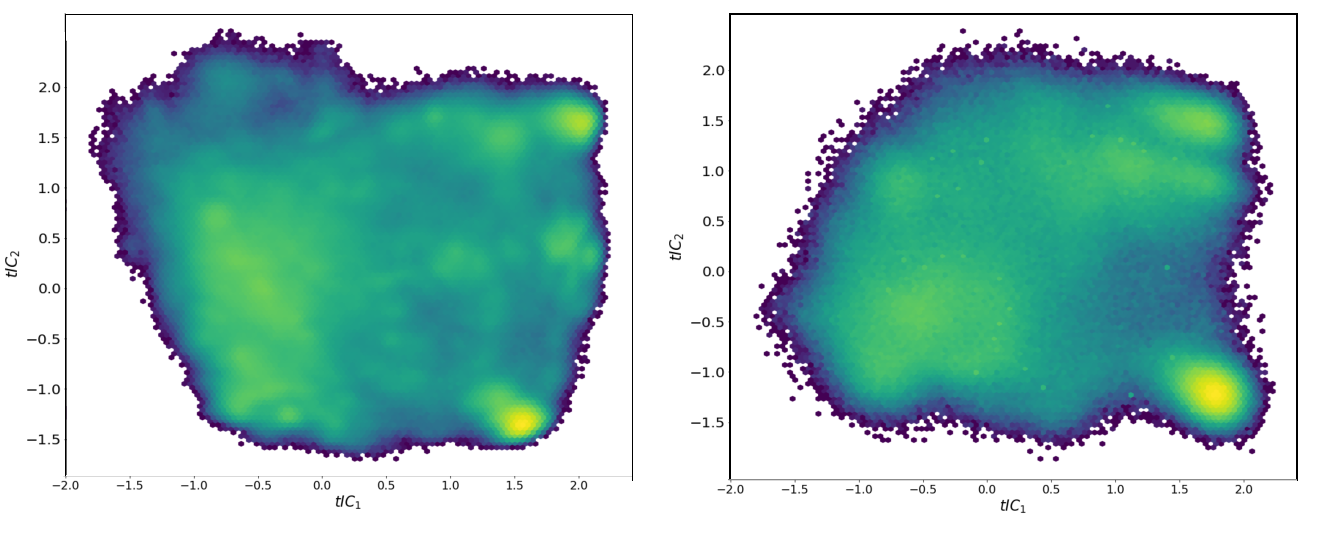
\includegraphics[scale=0.75]{Figures/SI/tica_compare.pdf}
\caption{Side-by-side comparison of MSMs constructed from
protein $C_{\alpha}$ and $C_{\beta}$ pair distances (left), and solvent shell features
(right), projected onto the first and second tICA components.}
\label{fig:tica_compare}
\end{figure}



\begin{figure}[h!]
\centering
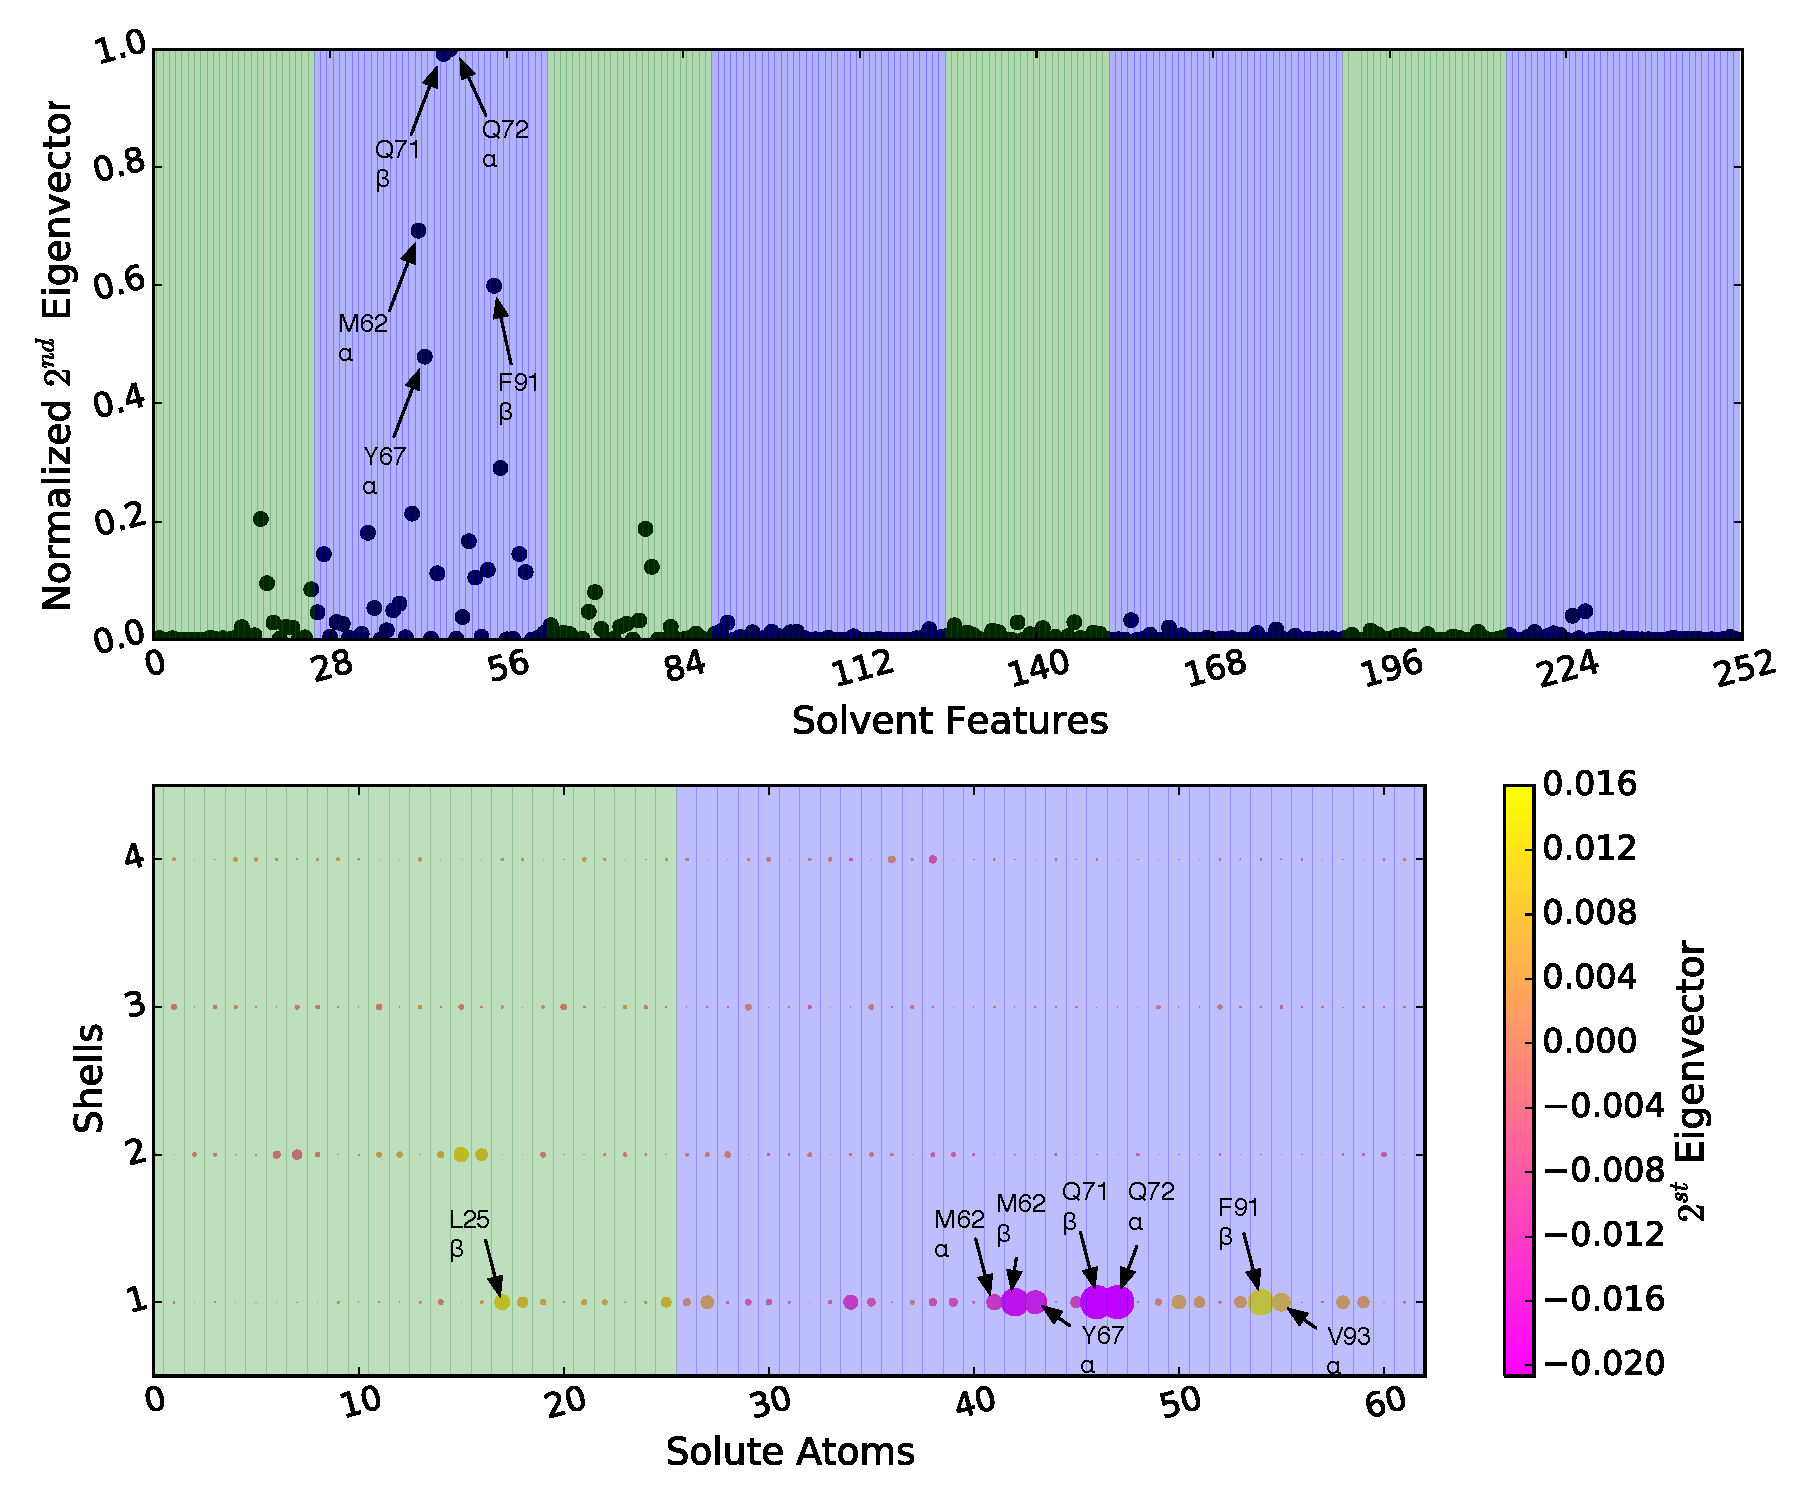
\includegraphics[scale=0.5]{Figures/SI/Solvent_Shell_Feature_Eigen_2}
\caption{\textbf{Solvent shells around key residues contribute to the slowest motions.} (Top) The degree of contribution for each solvent shell. Significant slow-dynamical solvent features are labeled by carbon atom and residue to which it belongs. The green and blue slices denote groups of residues for p53 and MDM2, respectively. (Bottom)  The second eigenvector revealed first shell (0-3 Å) of Methionine, M62 ($\beta$), Q71 ($\beta$), Q72 ($\alpha$), Phenylalanine, F91 ($\beta$) of MDM2 as well as Leucine, L25 ($\beta$), K24 ($\beta$) of p53 as the features contributing to theslowest motions.}
\label{fig:2nd_eigenvector}
\end{figure}


\begin{figure}[h!]
\centering
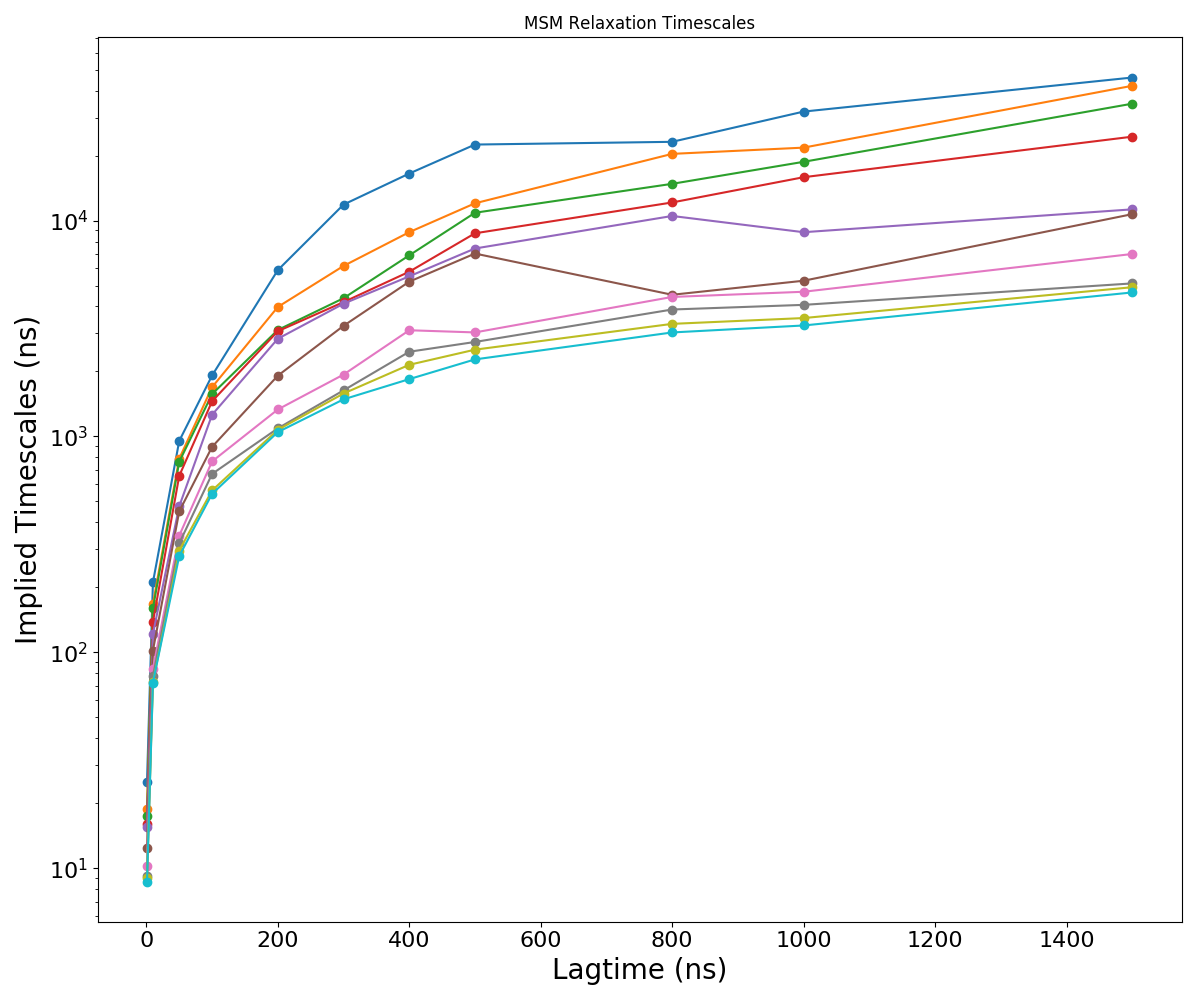
\includegraphics[scale=0.5]{Figures/Implied_timescales/solvent_lag_50_clusters_600.png}
\caption{Top ten implied timescales from the MSM built from solvent features.
}
\label{fig:implied_timescales}
\end{figure}





\subsubsection{Movies}


RUN9\_CLONE70: (531 ns)

{[}This movie is the overlaid trajectory in Figure 4.{]}

\#RUN7\_CLONE41: (271 ns)

This bound-unfolded trajectory shows W23 (yellow) pointing into the page
when the position of the trajectory trace contains a negative tIC2
value. Likewise, tIC1 is also negative, and the surface buckles inside
the hydrophobic pocket leaving a large cavity. This cavity represents a
high volume of water inside the pocket.

Here, we can see that movement along tIC1 correlates to the distance
from the pocket i.e., displacement of water inside the pocket. The helix
begins to coil at S20 of p53 at 193 ns (00:06) pulling F19 (light green)
closer to the pocket, simultaneously increasing tIC1 on the tICA
landscape. The maximum tIC1 value correlates to the instant (232 ns) W23
and F19 both enter the pocket.

\#RUN13\_CLONE53: (2001 ns)

During the first 20.0 ns the conformation of p53 is folded-unbound. This
particular trajectory is very interesting, in that, when W23 enters the
pocket, it's unable to lock into place due to its crooked positioning
(00:15).

Eventually, large surface cavities begin to form, and W23 gets jostled
out and performs a 360° turn at 41.1 ns (00:16). The helix stabilizes
when W23 and F19 are comfortable in the pocket.

\#RUN15\_CLONE32: (851 ns)

\#RUN18\_CLONE96: (216 ns)

This short trajectory

\#RUN24\_CLONE68: (321 ns)






\end{document}




% Overleaf Notes: {{{
%\section{Introduction}
%\subsection{Bayesian framework for inference}

%\color{red}
%\begin{itemize}
%    \item RR: 
%    \item 
%\end{itemize}
%\color{black}


%\begin{equation}
%P(X|D) \propto Q(D|X) P(X)
%\label{eq:bayes}
%\end{equation}

%\paragraph{Reference potentials.}
%The correct implementation of reference potentials is an important advantage of the BICePs algorithm. The experimental data used to construct the %likelihood function comes from some set of ensemble-averaged experimental observables $\mathbf{r} = (r_1, r_2, ..., r_N)$. Such observables are %low-dimensional projections of some high-dimensional state space $X$, and therefore these restraints in the space of observables need to be treated as %\textit{potentials of mean force}.\cite{Olsson:2013gq,Olsson:2011kl,Hamelryck:2010dea}

%\subsection{Restraint}
%The \verb|Restraint| class initializes all necessary functions to construct numpy array containing information for BICePs sampling. As a parent class, %it also includes child classes for different experimental restraints. Upon initialization, the algorithm will collect all input raw data and %corresponding experimental values for each experimental observable in each state. Meanwhile, $\chi^2$ values and reference potentials (see Theory) for %each restraint are computed at this step. 

%%%%%%%%%%%%%%%%%%%%%%%%%%%%%%%%%%%%%%%%%%%%%%%%%%%%%%%%%%%%%%%%%%%%%%%%%%%%%%%%%%%%%%%%%%%%%%%%%%%%%%%%%%%%%%%%%%%%%%%%%%%%%%%%%%%%%%%%%%%%%%%%%%%%%%%%%%%%%%%%%%%%%%
%\begin{equation}
%P(X | D) \propto\left[\frac{Q(\mathbf{r}(X) | D)}{Q_{\text { ref }}(\mathbf{r}(X))}\right] P(X)
%\label{eq:ref}
%\end{equation}

%%%%%%%%%%%%%%%%%%%%%%%%%%%%%%%%%%%%%%%%%%%%%%%%%%%%%%%%%%%%%%%%%%%%%%%%%%%%%%%%%%%%%%%%%%%%%%%%%%%%%%%%%%%%%%%%%%%%%%%%%%%%%%%%%%%%%%%%%%%%%%%%%%%%%%%%%%%%%%%%%%%%%
%\begin{figure}[h!]
%\centering
%\includegraphics[scale=0.5]{ref_potentials.pdf}
%\caption{A highly informative distance restraint has an experimental likelihood that differs significantly from its reference distribution.}
%\label{fig:ref_potentials}
%\end{figure}
%%%%%%%%%%%%%%%%%%%%%%%%%%%%%%%%%%%%%%%%%%%%%%%%%%%%%%%%%%%%%%%%%%%%%%%%%%%%%%%%%%%%%%%%%%%%%%%%%%%%%%%%%%%%%%%%%%%%%%%%%%%%%%%%%%%%%%%%%%%%%%%%%%%%%%%%%%%%%%%%%%%%%

%\begin{minted}
%[frame=lines,
%framesep=2mm,
%baselinestretch=1.2,
%fontsize=\small,%\footnotesize,
%linenos,
%xleftmargin=4em,
%xrightmargin=4em,]{python}
%from biceps import Preparation
%p = Preparation(scheme='noe', states=100, data_dir='NOE/*txt',
%    indices='atom_indice_noe.txt', exp_data='noe_distance.txt',
%    top='cineromycinB_pdbs/0.fixed.pdb')   
%p.write(out_dir='noe_J')
%\end{minted}

% }}}